\documentclass[12pt]{report}			% Začátek dokumentu
\usepackage{SP}							% Import stylu

\author{Jan Stejskal}
\title{Fotogrammetrie a její využití}
\date{14. února 2023}
\vedouci{Mgr. Karel Pazourek, Ph.D.}
\place{V Českých Budějovicích}
\skolnirok{2022/2023}
\logo{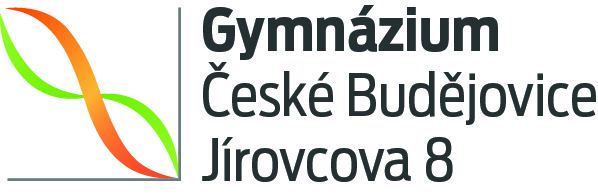
\includegraphics[scale=0.75]{logo_gymji.jpg}}

\begin{document}

	\mytitlepage						% Vygenerování titulní strany
	
	\prohlaseni{
		Prohlašuji, že jsem tuto práci vypracoval samostatně s vyznačením všech použitých pramenů.
	}	
	
	\abstrakt{Práce je zaměřena na přiblížení tématu fotogrammetrie. V teoretické části je vysvětleno, co je to fotogrammetrie, na jakém principu funguje ä za jakými účely je využívána. V praktické části je provedeno sestrojení 3D modelu objektu s pomocí fotogrammetrie.
	}{
	   Fotogrammetrie, fotografie, zeměměřictví, středový průmět			% Klíčová slova
	}
	
	\podekovani{
		Děkuji				% Poděkování
	}
	
	\tableofcontents\newpage			% Obsah
	
	
	
	
	\chapter*{Úvod}
	   Fotogrammetrie je samostatným vědním oborem geodézie a kartografie. Má bohatou historii a zvláště v posledních letech zažila rapidní rozvoj díky zlepšení počítačů a elektroniky. Stala se tak nejen hlavní mapovací metodou při státním mapování.
	
	
	\part{Teoretická část}
	
		\chapter{Fotogrammetrie}
			
			\section{Definice}
				Fotogrammetrie je vědní obor zabývající se získáváním informací z obrazových záznamů. Cílem fotogrammetrie je tedy rekonstrukce tvarů, měření rozměrů a určování polohy předmětů, které jsou zobrazeny na fotografických snímcích. Vstupem fotogrammetrie jsou fotografie a výstupem je obvykle mapa, výkres, měření nebo 3D model nějakého reálného objektu nebo scény. Mnoho map, které dnes používáme, je vytvořeno pomocí fotogrammetrie a fotografií pořízených z letadel. Název vznikl složením tří řeckých slov -- photos (světlo), gramma (záznam) a metron (měřit).
                

			\section{Historický vývoj}
                Teoretické počátky fotogrammetrie sahají dávno před vynález fotografie. 
                První zmínky o fotogrammetrii pochází z 11. století, kdy arabský učenec \textbf{Abu' Ali al-Hasan z Basry} popsal ve své práci princip fungování temné komory (camera obscura) pro pozorování obrazu zatmění Slunce. V době renesance \textbf{Leonardo da Vinci} (1452-1519) popsal a sestrojil dírkovou komoru, která umožňovala překreslování pozorovaného předmětu pomocí centrální projekce. Komora měla však malou světelnost, a proto se moc nevyužívala. \textbf{Giovanni Battista della Porta} poté popsal roku 1588 komoru vybavenou spojnou čočkou. Později byla za \textbf{Jana Keplera} zdokonalena jako \UIV{}camera clara, camera lucida, tím byl vlastně položen první skutečný základ fotogrammetrie. První praktické rekonstrukce perspektivních obrazů provedl \textbf{M.A.Cappeler} v Alpách, později \textbf{Charles-François Beatemps-Beaupré} pro pořízení plánu pobřeží ostrova Santa Gruz. Tyto metody však vyžadovaly ruční kresbu obrazů, značné malířské zkušenosti a nemohly dojít širšího uplatnění. Skoro upadly do zapomnění. Oživeny byly znovu po vynálezu fotografie (1839)\textbf{Josephem Nicéphorem Niépcem} a \textbf{Louisem Daguerrem}. Dva roky po tomto vynálezu slovenský vědec \textbf{Josef Maximilián Petzval} zkonstruoval moderní objektiv, zavedl do geometrické optiky exaktní výpočetní metody a přispěl tak k rozvoji fotogrammetrie. Za jednoho ze zakladatelů oboru se považuje \textbf{Aimé Laussedat}, podle jehož návrhu byl zkonstruován první fototeodolit (fotografický přístroj na získávání pozemních fotogrammetrických snímků). Jako první také využil fotografie země k výrobě topografických map.
                \\Pojem "fotogrammetrie" byl poprvé použit v článku architektonického časopisu v roce 1858 \textbf{Albrechtem Meydenbauerem}, který je považován za dalšího průkopníka fotogrammetrické dokumentace historických objektů a zároveň za zakladatele fotogrammetrie. Později byly nezávisle na sobě zkonstruované první prakticky využívané fototeodolity v letech 1865 v Itálii a 1895/1896 v Německu. Metoda průsekové fotogrammetrie, která do té doby byl užívaná, však měla velké nedostatky, hlavní v těžké identifikaci odpovídajících si bodů na snímcích. V roce 1901 byl podle návrhu \textbf{Carla Pulfricha} sestrojen stereokomparátor firmou Zeiss a tím došlo k rozvoji měřické metody nazývané stereofotogrammetrie, která byla přesnější než grafická průseková metoda. Stereokomparátor ale vyžadoval náročné výpočetní práce, došlo tedy k jeho zdokonalení a zjednodušilo se zpracování stereofotogrammetrických snímků. 
                \\S rozvojem letectví ve 20. století přišel také vznik letecké fotogrammetrie, kdy roku 1909 \textbf{Louis Blériot} přeletěl kanál La Manche a \textbf{Wilbur Wright} při letu pořizoval snímky. S příchodem 1. světové války fotogrammetrie zažila rozmach, byla využívána především pro vojenské sledovací účely. Za druhé světové války byla využívána v menším měřítku, velkého rozvoje dosáhla až po skončení konfliktu. Kolem roku 1960 vznikly přístroje, které umožňovaly částečně automatické vyhodnocení. S vývojem výpočetní techniky se také pomalu začalo přecházet na metody, které dříve nebylo možné využívat kvůli početní náročnosti. Překotný rozvoj v 80. letech poté umožnil vznik prvních digitálních systémů a mohla tak vzniknout digitální fotogrammetrie. Po roce 1995 se začaly používat nové digitální komory, které ještě zjednodušily snímání obrazu a zlevnily celý proces. Jednoduchá obsluha digitálních fotoaparátů a existence programů pro přímé vyhodnocení na základě běžných snímků vedly ke zpřístupnění digitální levné fotogrammetrie širší odborné veřejnosti. 

            %\section{Fotogrammetrie současnosti}


            \section{Principy fotogrammetrie}
                Vše se v podstatě odvíjí od konceptu triangulace. Triangulace zahrnuje pořízení snímků minimálně ze dvou různých míst. Tyto snímky vytvářejí zorné linie, které vedou z každého fotoaparátu do konkrétních bodů na fotografovaném objektu. Průsečík těchto linií se promítá do matematických výpočtů, které pomáhají vytvořit 3D souřadnice zadaných bodů.
                \\Zeměměřiči používají teodolity a triangulaci ke zjištění polohy bodu pomocí měření úhlů. Triangulační sítě mohou také pomoci s geodetickým systémem tím, že maximalizují přesnost.
                \\Je to vlastně podobný způsob, jakým pracují naše oči a vytvářejí hloubku. K vnímání hloubky dochází, když vidíme objekt z mírně odlišných úhlů, přičemž tyto úhly vycházejí z každého z našich očí. Náš mozek tyto dva obrazy zpracuje a vytvoří z nich jediný obraz, který dokážeme pochopit v procesu zvaném stereopse. Celý tento proces je podobný triangulaci.
                
            %\section{Středové promítání}
            
        \chapter{Dělení fotogrammetrie}
            \section{Podle polohy stanoviska}
                Jeden ze způsobů dělení fotogrammetrie je dělení podle toho, kde se nachází kamera, se kterou pořizujeme snímky.
                \subsection{Pozemní}
                    Při použití pozemní fotogrammetrie se stanovisko nepohybuje a je pevně spojeno se zemí. Snímky jsou pořizovány ze stanoviště na zemi s osou kamery rovnoběžnou se Zemí. Údaje o poloze kamery, jako jsou její souřadnice, jsou shromažďovány v okamžiku pořízení snímku. Přístroje používané pro pozemní snímkování jsou často teodolity, i když se někdy používají i běžné fotoaparáty. Pozemní fotogrammetrie pro geodetické účely obvykle vyžaduje méně prostředků a kvalifikovaných techniků, ale může trvat déle, než se pokryje velká část území.
                \subsection{Letecká}
                    Při letecké fotogrammetrii je kamera umístěna v letadle a obvykle je namířena svisle k zemi. Při letu letadla se pořizuje několik překrývajících se snímků země. Tradičně se používají letadla s pevnými křídly a posádkou, ale mnoho projektů se nyní realizuje pomocí bezpilotních letadel a dronů. Tradičně se tyto fotografie zpracovávaly v přístroji, který umožňoval operátorovi vidět dvě fotografie najednou ve stereo zobrazení, ale nyní se často zpracovávají pomocí automatizovaných stolních systémů.

                \subsection{Družicová}
                Ve větším měřítku se fotogrammetrie ve vesmíru provádí pomocí kamer umístěných na Zemi, na umělé družici nebo na Měsíci či jiné planetě. Ve skutečnosti byla fotogrammetrie považována za klíčovou součást výzkumu vesmíru již v 60. letech a díky technologickému pokroku se stala ještě aktuálnější. Dokáže nám poskytnout informace o struktuře mraků, vytvořit přesné mapy Země a shromáždit údaje o vzdálených planetách.
            \section{Podle počtu snímků}
                \subsection{Jednosnímková}
                Při jednosnímkové fotogrammetrii se k vyhodnocení využívá pouze samotný měřický snímek. Použití je však vhodné pouze pro objekty rovinné nebo blízké rovině. Jednosnímková metoda je tedy vhodná pro tvorbu fotoplánů například nepříliš členěných fasád domů.
                \subsection{Dvousnímková}
                Dvousnímková fotogrammetrie, většinou nazývána stereofotogrammetrie, je založená na stereoskopických principech, které umožňují vytvořit nebo zvýšit iluzi hloubky obrazu pomocí stereopse pro binokulární vidění. Binokulární vidění je založeno na principu, že můžeme levému a pravému oku předložit dva mírně odlišné obrazy zvlášť, přičemž mozek diváka tyto obrazy následně spojí a vytvoří vjem 3D vidění.
                \subsection{Vícesnímková}
                Pokud jsou osy záběrů snímků navzájem propojeny, hovoříme o vícesnímkovém prostorovém promítání. Technologicky se jedná o průsekovou fotogrammetrii, kdy pomocí prostorového protínání na dvou a více snímcích provádíme bodové vyhodnocení bez možnosti využití stereoskopického vjemu.
            \section{Podle způsobu zpracování}
                \subsection{Grafické metody}
                U této metody jsou všechny potřebné převody mezi souřadnicemi bodu na snímku a jeho polohou ve skutečnosti řešeny na základě deskriptivní geometrie bez nutnosti výpočtů.
                \subsection{Analogové metody}
                Dnes se již tyto metody nevyužívají. Mechanicky, opticky nebo kombinací obou byl vytvářen analogický stav jako při vlastním snímkování. Pro zpracování snímků bylo potřeba použít přesných a složitých vyhodnocovacích strojů, které v dnešní době již nejsou využívány.
                \subsection{Analytické metody}
                Souřadnice měřené na snímcích převedeme prostorovou transformací do geodetického systému pomocí analytických strojů nebo početně. Snímkové souřadnice se měří na poměrně jednoduchých strojích, transformace se provádí na libovolném výkonném počítači. Lze takto zpracovat v podstatě jakýkoliv snímek.
                \subsection{Digitální metody}
                Metoda funguje podobně jako analytická metoda. Využívá se digitální obraz a pro převod souřadnic pomocí transformace se také používá počítač. Souřadnice se měří ze snímku přímo v počítači.
            \section{Podle záznamu výsledků vyhodnocení}
                \subsection{Grafický}
                Výsledek vyhodnocení snímku je v tomto případě přímo graficky vyznačován na kreslicí stůl, který je připojený k vyhodnocovacímu stroji. Vzniká tak kartografický originál polohopisné případně i výškopisné složky mapy. Tato metoda se dnes ale nepoužívá, protože výsledek nejde dál přímo zpracovávat výpočetní technikou a nelze ho editovat či kvalitně reprodukovat.
                \subsection{Číselný}
                Základní způsob vyhodnocení, který spočívá v tom, že při analytickém nebo digitálním vyhodnocení automaticky registrujeme souřadnice jednotlivých bodů do paměti počítače nebo na jiné datové médium. Dále se zpracovávají buď přímo, nebo v jiném zpracovatelském systému do výsledné podoby. Výhodou této způsobu je přenositelnost výsledků, jejich ukládání a editace.
        \chapter{Výhody použití fotogrammetrie}
        Fotogrammetrie od svých počátků prošla řadou změn. V dnešní podobě je používána v mnoha oblastech, hlavně kvůli jejím vlastnostem, které usnadňují a urychlují postupy různých činností.
            \section{Bezkontaktní metoda měření}
            Fotogrammetrie využívá \textbf{bezkontaktní metody měření}. To znamená, že objekty, které fotíme, mohou být značně vzdáleny od místa snímkování. Tato vlastnost se projevuje zejména u nebezpečných nebo obtížně přístupných oblastí.
            \section{Krátká doba sběru dat}
            Další výhodou je \textbf{krátká doba sběru dat}, díky níž je doba snímkování podstatně kratší a většina práce se poté přesouvá do kanceláře. V porovnání s geodetickým zaměřováním je použití fotogrammetrie časově méně náročné, jednodušší a potřebné finanční náklady jsou také menší.
            \section{Práce u počítače}
            Pokud potřebujete informace znovu prozkoumat nebo vyhodnotit, nepotřebujete nákladnou práci v terénu. Pořízené fotogrammetrické snímky lze použít k opakovanému měření, čímž získáte nové informace pohodlným způsobem. Fotogrammetrie je skvělým způsobem, jak najít chybějící informace, například nedostatečné odstupy u příčných řezů.
            \section{Žádné narušení provozu}
            S využitím fotogrammetrie lze provádět silniční průzkumy, aniž by došlo k narušení provozu uzavřením jízdních pruhů nebo ohrožení terénního týmu. Vzhledem k tomu, že fotogrammetrie zohlední výškové údaje spolu s prvky silnice, lze je zobrazit v kanceláři, aniž byste je museli kontrolovat přímo v terénu.
            \section{Snadno popsatelné informace}
            Pomocí fotogrammetrie lze vyhodnotit souřadnice každého bodu v mapovacím poli bez jakéhokoli dalšího úsilí nebo nákladů. Jakmile jsou letecké snímky pořízeny, mohou být použity k předání nebo popisu informací státním, veřejným, dopravním divizím a dokonce i federálním úřadům.
        \chapter{Využití fotogrammetrie}
        Fotogrammetrie se používá v různých oborech, jako je mapování, strojírenství, architektura, výroba, policejní vyšetřování, kulturní dědictví, geologie, ale i ekologie, medicína, design nebo sport a dokonce i zábavní průmysl.
            \section{Mapování}
            Fotogrammetrie se používá při mapování terénu pomocí fotografií pořízených pomocí bezpilotních letadel, dronů, UAS (unnamed aerial system) nebo satelitů. Poskytuje snímky s vysokým rozlišením, vysokou přesností a mnohem kratší dobou zpracování. Fotogrammetrie umožňuje pořizovat vertikální i šikmé fotografie, které pomáhají získat přesný obraz terénu, což pomáhá při 3D mapování oblasti. Díky možnosti pořizování leteckých snímků je nyní snadné dostat se do obtížně přístupných oblastí a zmapovat terén, což zahrnuje dokonce i podvodní oblasti.
            \section{Stavební inženýrství}
            Fotogrammetrické techniky nabízejí podrobné informace o uspořádání povrchu pozemku, které mají zásadní význam pro stavební inženýrství. Použití této techniky je výhodné, protože k měření lze uvažovat neomezený počet bodů, které lze zpracovat automaticky během krátké doby. Pomocí snímků a 3D zobrazení území lze provést přesné rozvržení průběhu stavby.  Fotogrammetrické mapy také pomáhají při vytváření plánů rozvoje měst. Pomáhá dobře poznat terén, aby bylo možné přesně naplánovat silnice a cesty pro snadnější dopravu.
            \section{Film a zábavní průmysl}
            S digitalizací se natáčení filmů dramaticky změnilo. Díky úžasné animatronice vidíme filmy, které jsme si dříve nedokázali představit. Pomocí fotogrammetrie vznikají přesné 3D modely, které dávají filmařům volnost při tvorbě. Fotogrammetrie díky své schopnosti získat vysoce přesné rozměry zlepšila tvorbu realistických prostředí. Tato vlastnost fotogrammetrie se nyní hojně využívá při vytváření virtuálních prostředí pro hry, kde se připravují realistické situace pro zlepšení zážitku.
            \section{Sport}
            Fotogrammetrické techniky přinesly do sportovního průmyslu novou úroveň přesnosti. To platí zejména pro sportovní a rekreační aktivity, které jsou závislé na mapách. Sporty jako cyklistika, horolezectví, trekking, běžecké rallye, to vše závisí na přesnosti terénních map. Díky fotogrammetrickým terénním mapám získají sportovci velmi přesnou představu o náročnosti a rozmanitosti terénu, v němž budou závodit, a podle toho si naplánují svůj postup. Další nedávné využití fotogrammetrie ve sportu je ve virtuálním tréninkovém systému. V něm se fotogrammetrie využívá při sledování pohybů těla a dokáže zaznamenat i ten nejmenší posun v orientaci těla, což umožňuje identifikovat chyby a zlepšit svůj výkon o mnoho stupňů.
            \section{Kriminalistika}
            Díky rychlému a vysoce přesnému měření má fotogrammetrie obrovský potenciál pro využití ve forenzních vědách a studiích. Často se používá při dopravních nehodách a v případech nešťastných zranění, kdy je znalost nejmenších detailů nesmírně důležitá. Fotogrammetrie pomáhá zdokumentovat přesná měření, která jsou užitečná a přijatelná u soudu.
            \section{Medicína}
            Fotogrammetrie z blízka se používá při diagnostice a léčbě některých onemocnění a je široce využívána v biomedicínském výzkumu. Tato technika se používá především k měření obličeje a těla a k záznamu pohybů, konkrétně k měření zad, trupu a tvaru povrchu obličeje. Ačkoli by vás možná nenapadlo řadit lékařskou oblast do stejné kategorie jako zeměměřičství, 3D modely, které jsou výsledkem fotogrammetrické technologie, se hodí pro různé účely související se zdravotnictvím.
            \section{Vojenské průzkumy}
            Fotogrammetrie hraje roli také při sběru dat pro vojenské programy. Pro pochopení krajiny jsou nezbytné přesné geolokační modely s nízkou dobou zpracování. Letecké snímky a fotogrammetrické technologie mohou být použity dohromady a rychle vytvářet přesné 3D mapy bez lidského zásahu.
            \section{DPZ}
            Dálkový průzkum je získávání informací o objektu nebo jevu bez fyzického kontaktu s objektem. Tento termín se používá zejména pro získávání informací o Zemi a jiných planetách. Dálkový průzkum Země se používá v mnoha oborech, včetně geografie, zeměměřictví a většiny vědních oborů o Zemi (např. hydrologie, ekologie, meteorologie, oceánografie, glaciologie, geologie); má mimo jiné také vojenské, zpravodajské, obchodní, ekonomické, plánovací a humanitární využití.
            \\V současném užití se termín dálkový průzkum Země obecně vztahuje na použití satelitních nebo leteckých senzorových technologií k detekci a klasifikaci objektů na Zemi. Zahrnuje povrch, atmosféru a oceány, a to na základě šířených signálů (např. elektromagnetického záření). Lze jej rozdělit na "aktivní" dálkový průzkum (kdy je signál vysílán družicí nebo letadlem k objektu a jeho odraz je detekován senzorem) a "pasivní" dálkový průzkum (kdy je senzorem detekován odraz slunečního záření).

	\part{Praktická část}
        \chapter{Meshroom}
        \chapter{Příprava na rekonstrukci modelu}
        \chapter{Rekonstrukce modelu}


	\appendix
	\addcontentsline{toc}{part}{Apendix}
	
	\chapter*{Závěr}
	
		\lipsum[1]
	
	\nocite{*}
    \printbibliography					% Vytvoří seznam literatury
	\addcontentsline{toc}{chapter}{Bibliografie}
    \printglossary[title={Zkratky}]		% Vytvoří seznam zkratek
    \listoffigures						% Vytvoří seznam obrázků
    \listoftables						% Vytvoří seznam tabulek
    
    \begin{prilohy}
    	\pitem{Fotky z pokusů}
    	\eitem{Vlastní program}
    	\eitem{Dokumentace}
    	\eitem{Testovací data}
    \end{prilohy}
\end{document}